\documentclass[11pt]{article}
\usepackage[margin=1in]{geometry}
\usepackage{setspace}
\usepackage{iftex}
\usepackage{amsmath,amssymb}
\usepackage{graphicx}
\usepackage{enumitem}

\ifPDFTeX
  \usepackage[T1]{fontenc}
  \usepackage{newtxtext,newtxmath}
\else
  \usepackage{fontspec}
  \setmainfont{Times New Roman}
\fi

\setstretch{1.0}
\setlength{\parskip}{0.4em}
\setlength{\parindent}{0pt}
\pagenumbering{gobble}

\begin{document}

\begin{titlepage}
\centering
\vspace*{1in}
{\LARGE \textbf{Harnessing the Generative Quantum Eigensolver for Next-Generation Materials Design} \par}
\vspace{0.35in}
{\large \textit{Global Industry Challenge (GIC) 2026} \par}
\vspace{0.5in}
{\large Date: \today \par}
\vspace{0.3in}
\centering
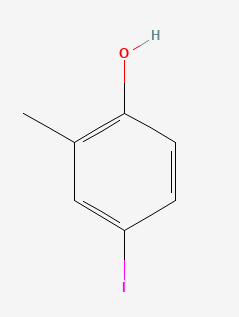
\includegraphics[width=0.35\textwidth]{../../img/4-Iodo-2-methylphenol.png}
\vspace{0.25em}

{\footnotesize Figure 1: 4-iodo-2-methylphenol (IMePh) structure. Source: PubChem.\par}
\vfill
{\large \textbf{Entangled Trio} \par}
\vspace{0.25in}
\begin{tabular}{lll}
Name & Profession & Role\\
\hline
Niraj Venkat & MS/MBA Student and Researcher & Project Manager / Team Coordinator \\
Muskan Aman & Electrical Engineer & Data / Technical Lead \\
Mackenson Polché & Posdoc Researcher in Energy Materials & Domain Expert
\end{tabular}
\vspace*{0.6in}
\end{titlepage}

\noindent\textbf{Executive Summary}\\
Our project targets a core bottleneck in advanced photoresist discovery: predicting EUV-driven excited-state and electron-emission behavior fast enough to guide candidate selection before expensive wet-lab cycles\footnote{Kharazi et al., "Quantum Simulations for Extreme Ultraviolet Photolithography," arXiv:2602.20234.}. We propose a hybrid Generative Quantum Eigensolver (GQE) workflow focused on 4-iodo-2-methylphenol (IMePh) as the anchor molecule and designed to extend to other structurally related photoresist candidates in the photolithography space. 

\noindent\textbf{High-level Overview of Proposed Solution}\\
We use a GQE-driven workflow to prepare a reference state, extract excited-state information, and compute Auger response signatures for IMePh and related candidates. We execute the following steps:
\begin{itemize}[leftmargin=*, itemsep=0pt, topsep=0pt, parsep=0pt, partopsep=0pt]
  \item \underline{Ground-State Preparation:} Sequence optimized state-preparation circuits for the IMePh ground state using a parameter-efficient Generative Quantum Eigensolver (GQE). By leveraging a Diffusion Transformer (DiT) rather than legacy autoregressive models, the architecture overcomes left-to-right bias to simultaneously capture non-local entanglement and global circuit topology. Output circuits are rigorously benchmarked for depth and fidelity against PySCF's exact Full Configuration Interaction (FCI) classical reference.
  \item \underline{Excited-State Extraction:} Apply the quantum self-consistent equation-of-motion (q-sc-EOM) method to obtain energies of the core-ionized $|\Psi_I\rangle$ and doubly-ionized $|\Psi_K\rangle$ states from the GQE reference.
  \item \underline{Auger Spectrum Calculation:} Compute the Auger transition rates using the one-centre approximation (OCA) to rank IMePh and related candidates by their EUV response signatures.
\end{itemize}
This gives a compact screening workflow that links circuit generation, excitation energies, and spectroscopy-based ranking.

\noindent\textbf{Technical Approach}\\
For each molecule, we construct an electronic Hamiltonian, map it to qubits (Jordan--Wigner), and evaluate learned circuit sequences:
\begin{equation*}
\rho(\mathbf{j}) = U_{j_L}\cdots U_{j_1}\,\rho_0\,U_{j_1}^{\dagger}\cdots U_{j_L}^{\dagger},
\qquad
E(\mathbf{j}) = \mathrm{Tr}\!\left[\hat{H}\rho(\mathbf{j})\right].
\end{equation*}
Minimizing the objective $\mathcal{L}_{\mathrm{GQE}} = \left(\sum_{i=1}^{L} w_{j_i} - E(\mathbf{j})\right)^2$ ensures a high-fidelity reference state. The total Auger decay rate $\Gamma_{KI}$ from a core-ionized state $I$ to a doubly-ionized state $K$ is calculated as\footnote{Keithley et al., "Auger Spectroscopy via Generative Quantum Eigensolver: A Quantum Approach to Molecular Excitations," https://arxiv.org/abs/2603.12859.}:
\begin{equation*}
\Gamma_{KI} = \sum_{l,m} 2\pi \left| \sum_{crs} \langle \phi_{Elm} \phi_c | \phi_r \phi_s \rangle R_{KI;csr} \right|^2
\end{equation*}
where $R_{KI;csr}$ is the transition reduced density matrix connecting the initial and final states. 

Our hybrid stack uses PennyLane's \verb|qml.qchem| for Hamiltonian construction and CUDA-Q for state-vector simulation. $\Gamma_{KI}$ are calculated via classical post-processing using the OCA and OpenMolcas atomic integrals. Our results are validated against classical PySCF FCI baselines, or Selected CI for larger candidate molecules.

\noindent\textbf{Projected Industry Impact}\\
For semiconductor stakeholders, this hybrid workflow accelerates photoresist screening by bypassing the exponential scaling limits of classical methods for core-electron decay processes. By producing physics-grounded rankings for EUV absorption and subsequent electron emission, it enables faster candidate prioritization before committing to expensive wet-lab synthesis. This repeatable screening tool significantly reduces development cycles and improves R\&D capital efficiency in next-generation lithography.

\end{document}
